\chapter{Anàlisi de la sostenibilitat i implicacions ètiques del Treball}
\section{Impacte ambiental}
\par Amb l'objectiu d'analitzar el possible impacte ambiental d'aquest treball, s'ha considerat la petjada ecològica directa i indirecta de les implicacions que pot tenir la realització d'aquest treball. 
\par Una de les mesures que s'han pres per reduir l'impacte ambiental, ha sigut reutilitzar components electrònics en desús d'anteriors projectes i utilitzar una placa de desenvolupament que ha sigut utilitzada per altres estudiants per acomplir el treball de fi de grau com el present. A més a més, materials com cables unifilars i una protoboard s'han utilitzat per a l'aplicació de la font d'àudio, els quals són materials que d'acabada la vida útil del projecte, es podràn reutilitzar per altres projectes. Per últim, les eines que s'han utilitzat en el desenvolupament del treball com el multímetre i l'oscil·loscopi, són propietat de la universitat i han sigut utilitzats només el temps que s'ha necessitat per la validació del projecte, permetent que altres estudiants de l'EEBE puguin fer-ne un ús similar.
\par Indirectament, la utilització de certs components com la placa de desenvolupament Nexys4 o la targeta ESP32, inclouen ICs que s'han produit a escala industrial. La producció a gran escala d'aquests components tenen una petjada ecològica associada que és rellevant en la lluita contra el canvi climàtic. Concretament, en \cite{FtprntEco} es fa un estudi detallat de la petjada ecològica per l'extracció de materials semiconductors. Es calcula que pel 2030 les emissions d'aquesta indústria es multiplicarien per 4 en els millors dels casos, superant les produides per altres indústries com la metalúrgica o d'aviació.
\begin{figure}[H]
    \centering
    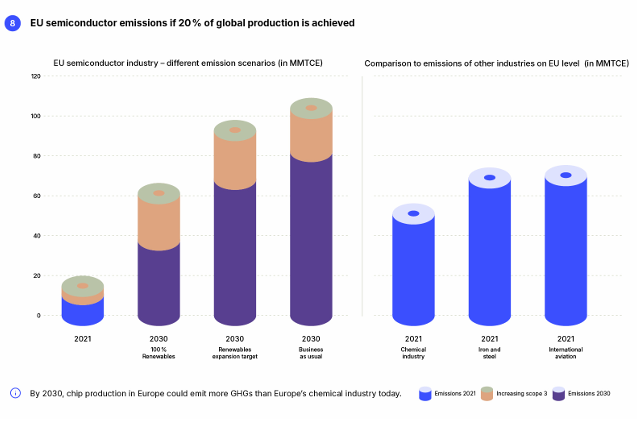
\includegraphics[width=0.25\linewidth]{Images/graf_ambienta.png}
    \caption{A l'esquerra predicció de les emissions de gasos d'efecte hivernacle de l'Indústria de producció de Semiconductors. A la dreta, les emissions de gasos produides per la indústria química, metal·lúrgica i d'aviació.\cite{FtprntEco}}
    \label{figGrafhivern}
\end{figure}
\par AMD, l'empresa fabricant de la FPGA utilitzada en la implementació d'aquest treball, publica annualment informes dels avenços en la reducció de la emissió de gasos d'efecte hivernacle, amb l'objectiu de contribuir a complir els objectius de l'agenda 2030.\cite{AMDGHG}

\chapter{Pressupost del treball}
\section{Cost retributiu}
\par Per estimar els costos de l'elaboració d'aquest treball cal considerar el temps invertit, les persones involucrades i les respectives retribucions per hores. En l'elaboració d'aquest projecte han participat l'autor del treball i el corresponent tutor en matèria d'assessorament. Conforme \cite{BOEsal}, el SMI per un enginyer tècnic amb graduat universitari és 22224,26 \euro per un any de treball a jornada completa i 14 pagues. S'assigna doncs una retribució horària per l'autor d'aquest treball de 10,68 \euro/h. La realització d'aquest treball implica la dedicació mínima de 24 ECTS, que amb l'equivalència de 25 h/ECTS resulta en 600 hores de dedicació total. 
\begin{table}[H]
    \centering
    \begin{tabular}{ | c | c | c | c |}
    \hline
    \textbf{Cost Retributiu}     &  \textbf{Hores dedicades} & \textbf{Sou}& \textbf{Cost total}\\ [2ex] \hline
    Cost mà d'obra   & 600 h & 10,68 & 6408 \euro \\ \hline
    Cost assessorament  & 9 h & 20 & 180 \euro \\ \hline
    \textsc{TOTAL}    &  -  & - & 6588 \euro \\ \hline
    \end{tabular}
    \caption{Costos en concepte de retribució dels implicats en la realització del present treball.}
    \label{taula_salaris}
\end{table}

\section{Costos dels materials}
\par La implementació física del treball ha requerit un seguit de components i eines amb un cost econòmic. A la taula \ref{taula_material} es detallen els costos dels materials emprats en el desenvolupament del treball. 
\begin{table}
    \centering
    \begin{tabular}{ | c | c | }
    \hline
    \centering
    \textbf{Material}     &  \textbf{Preu de mercat}\\ [2ex] \hline
    \centering
    Targeta ESP32-WROOM    &    11,50 \euro \\ \hline
    \centering
    Adapatador targeta $\mu$SD    &    3,85 \euro \\ \hline
    \centering
    Targeta $\mu$SD    &    3,50 \euro \\ \hline
    \centering
    Mòdul alimentació de 5V i 3,3V    &    4,50 \euro \\ \hline
    \centering
    Placa de desenvolupament NEXYS4    &    412 \euro \\ \hline
    \centering
    Kit protoboards i cables    &    3 \euro \\ \hline
    \centering
    Auricolars amb entrada jack de 3.5 mm    &    7 \euro \\ \hline
    \centering
    \textsc{TOTAL}    &    445,35 \euro \\ \hline
    \end{tabular}
    \caption{Costos en material utilitzat per la implementació del treball.}
    \label{taula_material}
\end{table}

\section{Costos de les eines}
\par A continuació, es procedeix a fer una valoració econòmica de les eines que s'han utilitzat i el temps que s'han emprat. En el còmput global del pressupost del treball, només es considerarà l'amortització. A la taula següent es desglossen les eines emprades:
\begin{table}[H]
    \centering
    \begin{tabular}{ | c | c | c | c | c |}
    \hline
    \centering
    \textbf{Eines}     &  \textbf{Preu de mercat} & \textbf{Vida útil}  & \textbf{Temps d'ús} & \textbf{Amortització}\\ [2ex] \hline
    \centering
    Ordinador Portàtil    &  1000 \euro &  10000 h  &  540 h  &  54 \euro\\ \hline
    \centering
    Multímetre    &    20 \euro &  1000 h  &  10 h  &  0.2 \euro\\ \hline
    \centering
    Oscil·loscopi    &    3270 \euro &  10000 h  &  10 h  &  3,27 \euro\\ \hline
    \centering
    Estació de soldadura   &    420,75 \euro &  5000 h  &  15 min  &  0,02 \euro\\ \hline
    \centering
    \textsc{TOTAL}    &    - &  -  &  -  &  57,49 \euro\\ \hline
    \end{tabular}
    \caption{Costos d'amortització de les eines emprades pel desenvolupament del treball.}
    \label{taula_eines}
\end{table}

\par En el disseny de les etapes de filtratge de l'amplificador de classe D digital s'ha emprat el programa MATLAB\textsuperscript{\tiny\textregistered}, i aquest té un cost de llicència de 119 \euro \ com a preu de partida.\cite{MATLABlic}

\section{Pressupost final}
\par Finalment, es presenta la taula \ref{taula_pressupost} on s'engloben els costos totals del treball implementat.
\begin{table}[H]
    \centering
    \begin{tabular}{ | c | c | }
    \hline
    \centering
    \textbf{Concepte}     &  \textbf{Cost}\\ [2ex] \hline
    \centering
    Cost Retributiu    &    6588 \euro \\ \hline
    \centering
    Costos dels materials    &    445,35 \euro \\ \hline
    \centering
    Costos de les eines \& llicències   &    176,49 \euro \\ \hline
    \centering
    \textsc{TOTAL}    &    7209,84 \euro \\ \hline
    \end{tabular}
    \caption{Pressupost total del treball realitzat.}
    \label{taula_pressupost}
\end{table}